\documentclass[a4paper,12pt,twoside]{article}
\usepackage[utf8]{inputenc}
\usepackage{graphicx}
\usepackage{subfig}
\usepackage[table,xcdraw]{xcolor}
\usepackage{amsmath,amssymb,amsfonts,bm}
\usepackage[bottom=2cm,top=2cm,left=2.0cm,right=2.0cm]{geometry}
\usepackage{float}
\usepackage[portuges]{babel}
\usepackage{indentfirst}
\usepackage[colorlinks=true, allcolors=black]{hyperref}
\usepackage[alf]{abntex2cite}
\usepackage[export]{adjustbox}
\usepackage{afterpage}
\usepackage{multicol}
\usepackage{multirow}
\usepackage{textcomp}
\usepackage{ dsfont }
\usepackage{listings}

\usepackage{fancyhdr}
\pagestyle{fancy}
\fancyhf{}
\fancyhead[RO,LE]{\nouppercase{\emph\leftmark}}
\fancyhead[LO,RE]{\emph \thepage}
\renewcommand{\sectionmark}[1]{\markboth{#1}{}}

\newtheorem{teo}{Teorema}[section]
\newtheorem{lema}[teo]{Lema}
\newtheorem{cor}[teo]{Corolário}
\newtheorem{prop}[teo]{Proposição}
\newtheorem{defi}{Definição}
\newtheorem{exem}{Exemplo}

\usepackage{color}

\definecolor{codegreen}{rgb}{0,0.6,0}
\definecolor{codegray}{rgb}{0.5,0.5,0.5}
\definecolor{codepurple}{rgb}{0.58,0,0.82}
\definecolor{codeyellow}{rgb}{0.67,0.67,0.0}
\definecolor{backcolour}{rgb}{0.95,0.95,0.92}

\lstset{
language=R,   % R code
literate=
{á}{{\'a}}1
{à}{{\`a}}1
{ã}{{\~a}}1
{é}{{\'e}}1
{ê}{{\^e}}1
{í}{{\'i}}1
{ó}{{\'o}}1
{õ}{{\~o}}1
{ú}{{\'u}}1
{ü}{{\"u}}1
{ç}{{\c{c}}}1
}
\lstdefinestyle{mystyle}{
    language=R,
    backgroundcolor=\color{backcolour},   
    commentstyle=\color{codegreen},
    keywordstyle=\color{blue},
    emphstyle=\color{codeyellow},
    numberstyle=\scriptsize\color{black},
    stringstyle=\color{codegreen},
    basicstyle=\rmfamily\scriptsize,
    breakatwhitespace=false,         
    breaklines=true,                 
    captionpos=b,                    
    keepspaces=true,                 
    numbers=left,                    
    numbersep=6pt,                  
    showspaces=false,                
    showstringspaces=false,
    showtabs=false,                  
    tabsize=2
}

\lstset{style=mystyle}

\begin{document}
\newgeometry{bottom=2.0cm,top=1cm,left=2.0cm,right=2.0cm}
\thispagestyle{empty}
	\begin{figure}[htb!]
		\begin{flushright}
			
\includegraphics[scale=.3]{UNICAMP_logo.jpg} 
		\end{flushright}
	\end{figure}
	\vspace{-3.5cm}
	\hspace{1.5cm}
	\begin{flushleft}
	\begin{minipage}{15cm}
	\textbf{IMECC-UNICAMP\\
	Atividade 1 - Métodos computacionais}\\
	Professor: Dr. Guilherme Ludwig\\
	Vitor Macedo Rocha RA: 216394
	\end{minipage}
	\end{flushleft}
\noindent\rule{17cm}{0.4pt}

\section{Distribuições condicionais completas e implementação Gibbs}\label{gibbs}

Considere $\mathbf{p}=[p_{1},...,p_{14}]^{\top}$, $\mathbf{x}=[n_1,...,n_{14},m_1,...,m_{14}]^{\top}$ e $\mathbb{B}=\{0,1,2,...,N\}$, temos que a verosimilhança e as distribuições a priori são dadas por
\begin{align}
&\mathcal{L}(N,\mathbf{p}|\mathbf{x})\propto \frac{N!}{(N-r)!}\prod_{i=1}^{14}p_{i}^{n_i}(1-p_i)^{N-n_i}\mathds{I}(N \in \mathbb{N})\mathds{I}(p_i \in [0,1])\mathds{I}(r \in \mathbb{B})\\
&\pi(N)=\frac{e^{-\lambda}\lambda^{N}}{N!} \mathds{I}(N \in \mathbb{N})\\
&\pi(p_i)=\mathds{I}(p_i \in [0,1]) , i=1,2,...,14.
\end{align}

A seguir vamos derivar a distribuição condicional completa de $N|\mathbf{p,x}$. Note que $\mathds{I}(N \in \mathbb{N})\mathds{I}(p_i \in [0,1])\mathds{I}(r \in \mathbb{B})=\mathds{I}(N \in {r,r+1,...})\mathds{I}(p_i \in [0,1])$, pois $\mathds{I}(r \in \mathbb{B})=\mathds{I}(N \in \{r,r+1,...\})$.

\begin{align*}
\pi(N|\mathbf{p,x})&\propto \mathcal{L}(N,\mathbf{p}|\mathbf{x}) \pi(N)\\
&= \frac{N!}{(N-r)!}\prod_{i=1}^{14}p_{i}^{n_i}(1-p_i)^{N-n_i}\mathds{I}(N \in \{r,r+1,...\})\mathds{I}(p_i \in [0,1])\frac{e^{-\lambda}\lambda^{N}}{N!} \mathds{I}(N \in \mathbb{N})\\
&=\frac{e^{-\lambda}\lambda^{N}}{(N-r)!}\prod_{i=1}^{14}p_{i}^{n_i}(1-p_i)^{N}(1-p_i)^{-n_i}\mathds{I}(N \in \{r,r+1,...\})\mathds{I}(p_i \in [0,1])\\
&=\frac{e^{-\lambda}\lambda^{N}}{(N-r)!}\prod_{i=1}^{14}\left[p_{i}^{n_i}\right]\prod_{i=1}^{14}\left[(1-p_i)^{N}\right]\prod_{i=1}^{14}\left[(1-p_i)^{-n_i}\right]\mathds{I}(N \in \{r,r+1,...\})\mathds{I}(p_i \in [0,1])\\
& \propto \frac{e^{-\lambda}\lambda^{N}}{(N-r)!}\left[\prod_{i=1}^{14}(1-p_i)\right]^{N}\mathds{I}(N \in \{r,r+1,...\})\mathds{I}(p_i \in [0,1])\\
& = \frac{e^{-\lambda}\left[\lambda\prod_{i=1}^{14}(1-p_i)\right]^{N}}{(N-r)!}\mathds{I}(N \in \{r,r+1,...\})\mathds{I}(p_i \in [0,1])\frac{e^{-\lambda\prod_{i=1}^{14}(1-p_i)}}{e^{-\lambda\prod_{i=1}^{14}(1-p_i)}}\\
& \propto \frac{\exp\{-\lambda\prod_{i=1}^{14}(1-p_i)\}\left[\lambda\prod_{i=1}^{14}(1-p_i)\right]^{N}}{(N-r)!}\mathds{I}(N \in \{r,r+1,...\})\mathds{I}(p_i \in [0,1])\\
& \propto \frac{\exp\{-\lambda\prod_{i=1}^{14}(1-p_i)\}\left[\lambda\prod_{i=1}^{14}(1-p_i)\right]^{N-r}}{(N-r)!}\mathds{I}(N \in \{r,r+1,...\})\mathds{I}(p_i \in [0,1])\\
& = \frac{\exp\{-\lambda\prod_{i=1}^{14}(1-p_i)\}\left[\lambda\prod_{i=1}^{14}(1-p_i)\right]^{N-r}}{(N-r)!}\mathds{I}(N-r \in \mathbb{N})\mathds{I}(p_i \in [0,1])\\
\end{align*}
Portanto
\begin{equation}\label{piN}
\pi(N|\mathbf{p,x})\propto \frac{\exp\{-\lambda\prod_{i=1}^{14}(1-p_i)\}\left[\lambda\prod_{i=1}^{14}(1-p_i)\right]^{N-r}}{(N-r)!}\mathds{I}(N-r \in \mathbb{N})\mathds{I}(p_i \in [0,1])
\end{equation}

Temos que $(N-r)|(\mathbf{p,x})\sim Poisson(\lambda\prod_{i=1}^{14}(1-p_i))$, identificado pelo \textit{kernel} apresentado em \ref{piN}.
\newpage
\restoregeometry
Agora vamos derivar a distribuição condicional completa de $p_i|N,\mathbf{x}, i=1,2,...,14$. Considere $\mathbf{p_{(i)}}=(p_1,p_2,...,p_{i-1},p_{i+1},...,p_{14}$, isto é, o vetor de parâmetros $\mathbf{p}$ sem o i-ésimo elemento.
\begin{align*}
\pi(p_i|N,\mathbf{p_{(i)},x})&\propto \mathcal{L}(N,\mathbf{p}|\mathbf{x}) \pi(\mathbf{p_{(i)}})\\
& = \frac{N!}{(N-r)!}\prod_{l=1}^{14}p_{i}^{n_l}(1-p_l)^{N-n_l}\mathds{I}(N \in \{r,r+1,...\})\mathds{I}(p_l \in [0,1])\left[\prod_{j\neq i}\mathds{I}(p_j \in [0,1])\right]\\
& = \frac{N!}{(N-r)!}\prod_{l=1}^{14}p_{l}^{n_l}(1-p_l)^{N-n_l}\mathds{I}(N \in \{r,r+1,...\})\mathds{I}(p_l \in [0,1])\\
& \propto p_i^{n_i}(1-p_i)^{N-n_i}\mathds{I}(p_i \in [0,1])\\
& = p_i^{(n_i-1)+1}(1-p_i)^{(N-n_i-1)+1}\mathds{I}(p_i \in [0,1])
\end{align*}
Podemos então identificar que $p_i|N,\mathbf{x} \sim \text{Beta}(n_i+1,N-n_i+1), i=1,2,...,14$ pelo kernel que apresentado acima. Chegamos a conclusão que 

\begin{align}
& (N-r)|(\mathbf{p,x})\sim Poisson(\lambda\prod_{i=1}^{14}(1-p_i))\\
& p_i|N,\mathbf{x} \sim Beta(n_i+1,N-n_i+1), i=1,2,...,14
\end{align}

Para avaliar a convergência para a distribuição estacionária, vamos gerar as 4 cadeias com diferentes pontos iniciais e avaliar visualmente se elas se misturam.

\begin{figure}[H]
  \centering
  \subfloat[\footnotesize{$p_1$}]{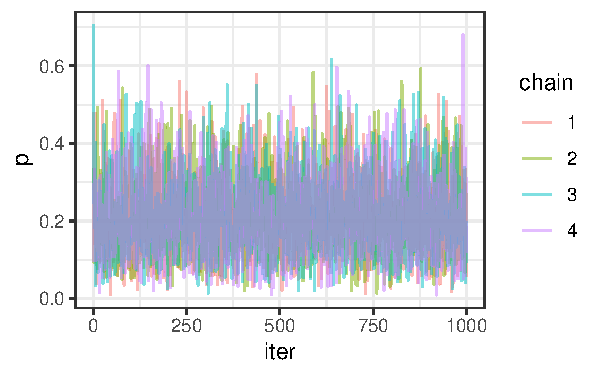
\includegraphics[width=8cm,height=5cm]{imgs/p1.pdf}}
  \subfloat[\footnotesize{$p_2$}]{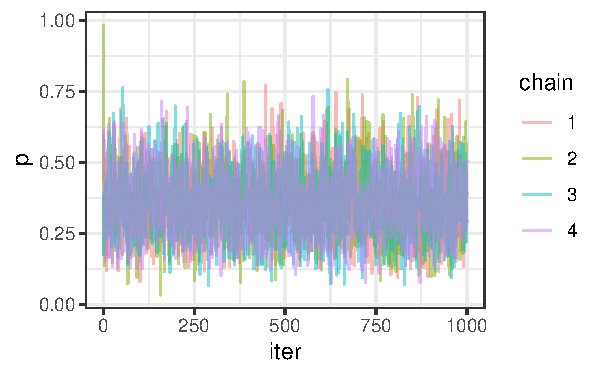
\includegraphics[width=8cm,height=5cm]{imgs/p2.pdf}} \\
  \subfloat[\footnotesize{$p_3$}]{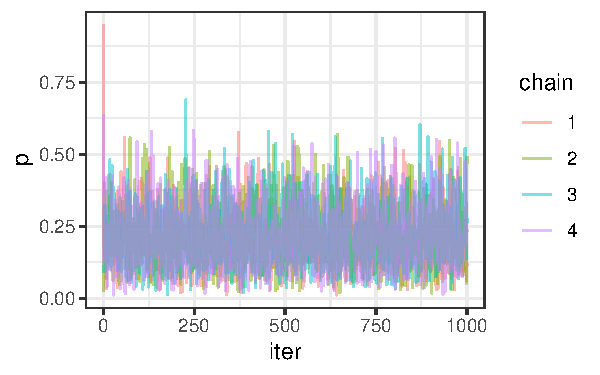
\includegraphics[width=8cm,height=5cm]{imgs/p3.pdf}}
  \subfloat[\footnotesize{$p_4$}]{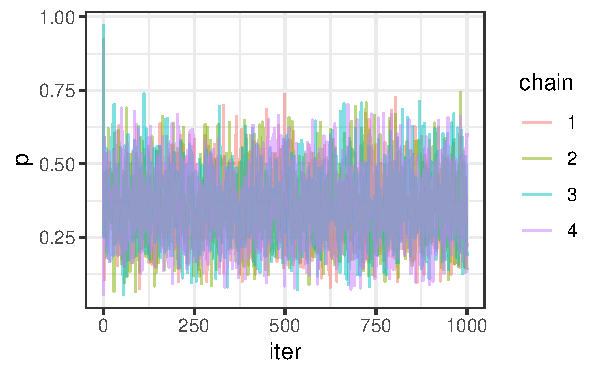
\includegraphics[width=8cm,height=5cm]{imgs/p4.pdf}}\\
  %
  \captionsetup{font=footnotesize,width=15cm}
  \caption{\small }
\end{figure}

\newpage
\begin{figure}[H]
  \centering
  \subfloat[\footnotesize{$p_5$}]{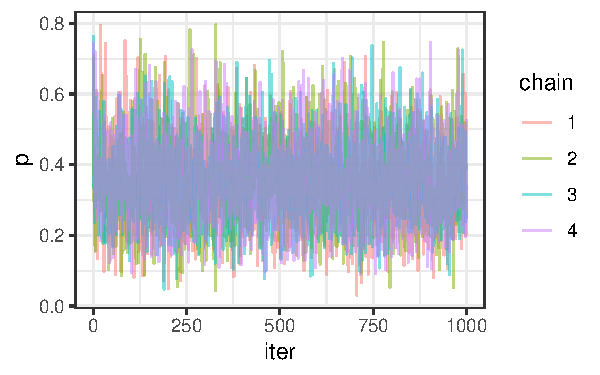
\includegraphics[width=8cm,height=5cm]{imgs/p5.pdf}}
  \subfloat[\footnotesize{$p_6$}]{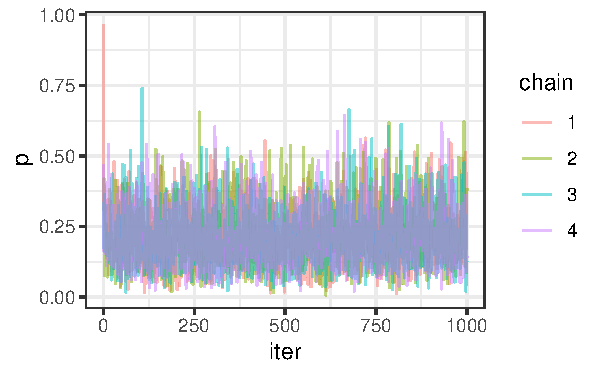
\includegraphics[width=8cm,height=5cm]{imgs/p6.pdf}} \\
  \subfloat[\footnotesize{$p_7$}]{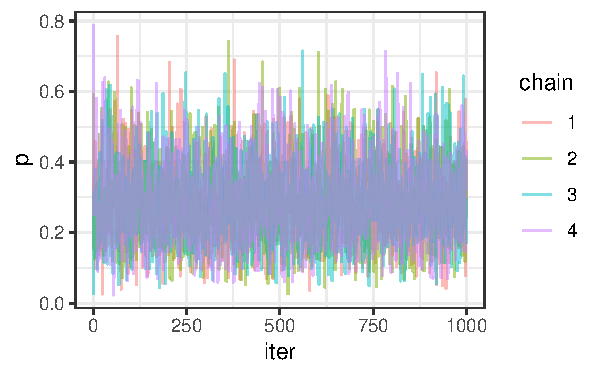
\includegraphics[width=8cm,height=5cm]{imgs/p7.pdf}}
  \subfloat[\footnotesize{$p_8$}]{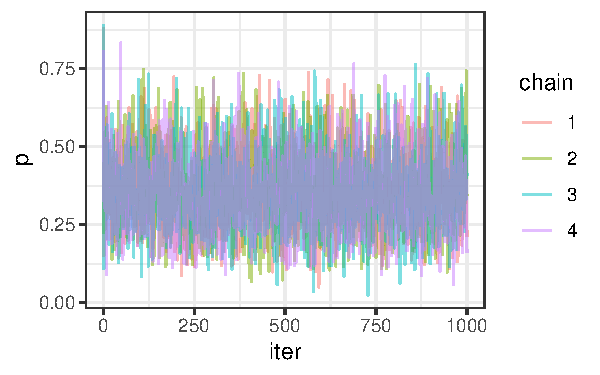
\includegraphics[width=8cm,height=5cm]{imgs/p8.pdf}} \\\subfloat[\footnotesize{$p_9$}]{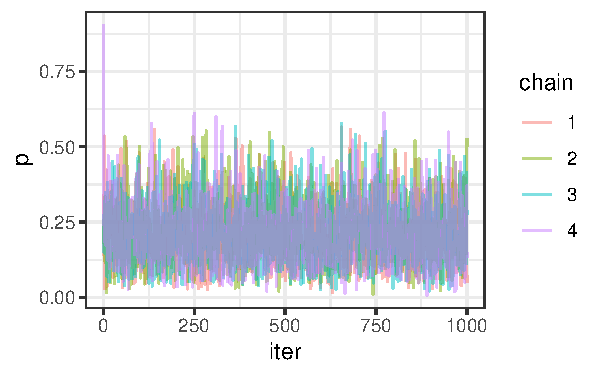
\includegraphics[width=8cm,height=5cm]{imgs/p9.pdf}}
  \subfloat[\footnotesize{$p_{10}$}]{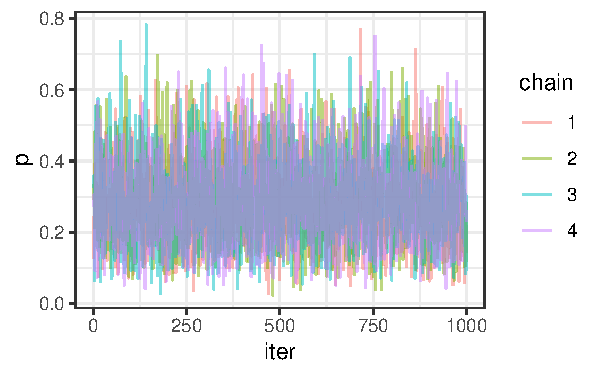
\includegraphics[width=8cm,height=5cm]{imgs/p10.pdf}} \\\subfloat[\footnotesize{$p_{11}$}]{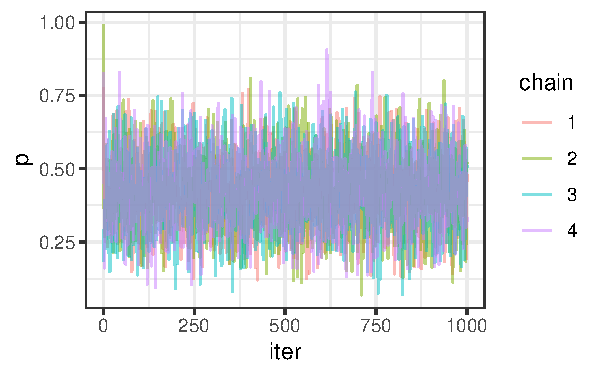
\includegraphics[width=8cm,height=5cm]{imgs/p11.pdf}}
  \subfloat[\footnotesize{$p_{12}$}]{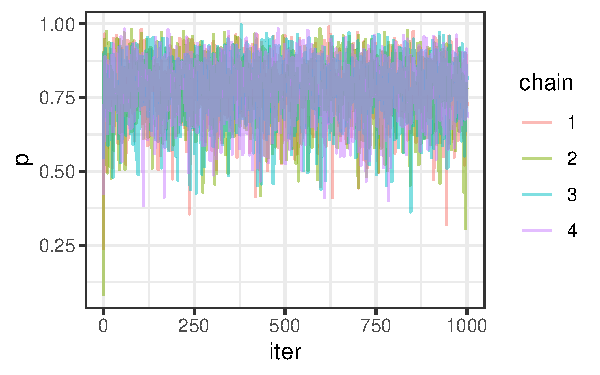
\includegraphics[width=8cm,height=5cm]{imgs/p12.pdf}} \\\label{a}
  %
  \captionsetup{font=footnotesize,width=15cm}
  \caption{\small }
\end{figure}

\newpage
\begin{figure}[H]
  \centering
  \subfloat[\footnotesize{N}]{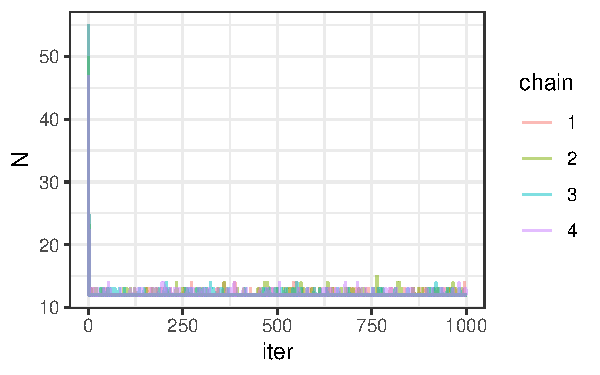
\includegraphics[width=8cm,height=5cm]{imgs/N.pdf}}
    \subfloat[\footnotesize{Auto correlação do parâmetro N.}]{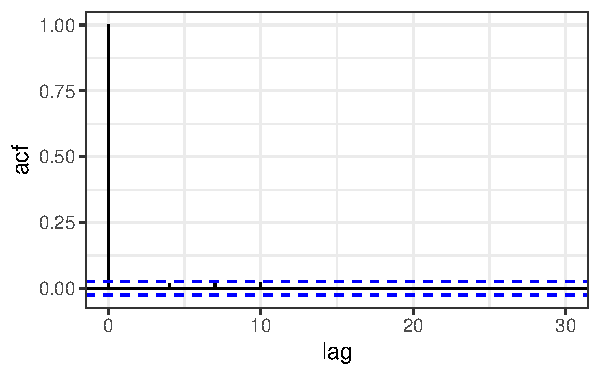
\includegraphics[width=8cm,height=5cm]{imgs/Nacf.pdf}}
  %
  \captionsetup{font=footnotesize,width=15cm}
  \caption{\small }
\end{figure}

Podemos ver que as cadeias para todos os parâmetros se misturaram, trazendo indícios da convergência para a distribuição estacionária. Além disso vemos pelo gráfico da autocorrelação da cadeia do parâmetro N que não precisamos realizar o processo de \textit{decorrelation} para garantir uma amostra pseudo-independente. Os gráficos de autocorrelação dos parâmetros $p_i,i=1,2,...,14.$ apresentaram um comportamento similar.

\begin{table}[ht]
\centering
\begin{tabular}{cccc}
  \hline
  Parâmetro & Média & Mediana & intervalo de credibilidade 95\% \\ 
  \hline
 N & 12.140 & 12.000 & [12;13] \\ 
p1 & 0.211 & 0.196 & [0.051;0.452] \\ 
p2 & 0.352 & 0.346 & [0.136;0.608] \\ 
p3 & 0.212 & 0.197 & [0.052;0.446] \\ 
 p4 & 0.355 & 0.348 & [0.139;0.604] \\ 
 p5 & 0.356 & 0.349 & [0.139;0.613] \\ 
 p6 & 0.213 & 0.199 & [0.05;0.456] \\ 
 p7 & 0.284 & 0.277 & [0.088;0.531] \\ 
 p8 & 0.356 & 0.347 & [0.137;0.614] \\ 
 p9 & 0.214 & 0.200 & [0.051;0.452] \\ 
p10 & 0.285 & 0.276 & [0.091;0.531] \\ 
 p11 & 0.426 & 0.419 & [0.187;0.684] \\ 
 p12 & 0.778 & 0.791 & [0.538;0.946] \\ 
p13 & 0.213 & 0.199 & [0.051;0.458] \\ 
 p14 & 0.427 & 0.425 & [0.188;0.678] \\ 
   \hline
\end{tabular}
\end{table}

\newpage
\section{Implementação \textit{Hamiltonian Monte Carlo}}
Como bem sabemos, o HMC \textit{sampler} não comporta suportes discretos pela fato de que a função que descreve a energia cinética há de ser derivável em relação a "trajetória" da cadeia. Por esse fato, optei por procurar uma solução na própria documentação do stan e acabei encontrando a opção de marginalização do parâmetro discreto.

Para realizar a implementação no R, procurei artigos na web que tratassem desse assunto e encontrei uma extensão do HMC chamado de \textit{Discontinuous Hamiltonian} Monte Carlo \cite{dhmc}. Nele é discutido também o porquê o HMC falha quando temos interesse em densidades alvo descontínuas, resumidamente a etapa da solução das equações diferenciais via \textit{leapfrog} apresenta uma instabilidade levando ao erro.

Outra ideia que tive foi utilizar a aproximação da distribuição poisson pela Normal, da seguinte maneira $Poisson(\lambda)\approx Normal(\mu=\lambda,\sigma^2=\lambda)$. Como essa última foi a solução mais simples que achei, vou implementar primeiro e se tiver tempo hábil tentarei implementar as outras.

\subsection{HMC via aproximação Poisson-Normal}

No gráfico a seguir podemos ver que a aproximação é realmente razoável.
\begin{figure}[H]
  \centering
  \subfloat[\footnotesize{}]{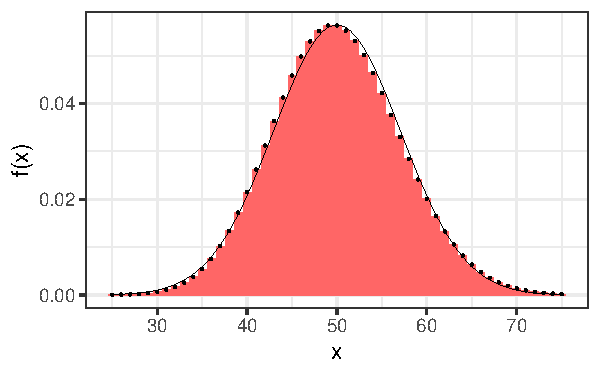
\includegraphics[width=8cm,height=5cm]{imgs/g1.pdf}}
  \subfloat[\footnotesize{}]{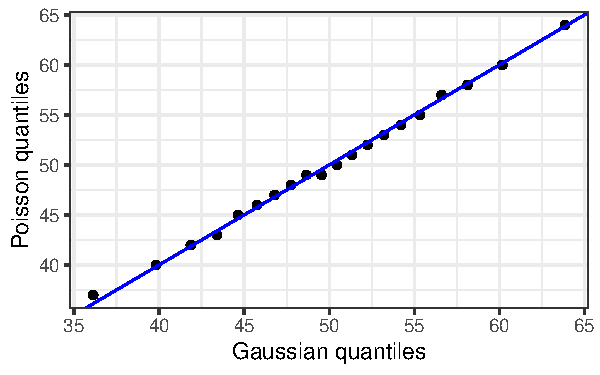
\includegraphics[width=8cm,height=5cm]{imgs/g2.pdf}}

  \captionsetup{font=footnotesize,width=15cm}
  \caption{\small Aproximação da distribuição $Poisson(\lambda=50)$ pela distribuição $Normal(\mu=50,\sigma^2=50)$.}
\end{figure}

A partir da verosimilhança apresentada em \ref{gibbs} e as distribuições a priori $\pi(N)\sim Normal(50,50)$ e $\pi(p_i)\sim U(0,1),i=1,2,...,14$. Obtemos a seguinte função proporcional a distribuição a posteriori.

\begin{align*}
\pi(N,\mathbf{p|x})\propto \left[\frac{N!}{(N-r)!}\prod_{i=1}^{14}p_{i}^{n_i}(1-p_i)^{N-n_i}\mathds{I}(p_i \in [0,1])\mathds{I}(r \in [0,N])\right] \times \pi(N) \times \pi(\mathbf{p}) 
\end{align*}

Precisamos então das quantidade referentes a "força cinética" $K(\bm{\rho})$ e "força potencial" $U(\mathbf{\bm{\theta}})$. Definimos, para $p_i \in [0,1], i=1,2,...,14$, sendo $\bm{\theta}=[N,p_1,...,p_14]$.
\newpage
\begin{align*}
&U(\mathbf{\bm{\theta}})=-\log(\pi(N,\mathbf{p|x}))\\
&-\left[\log(\Gamma(N+1)) - \log(\Gamma(N-r+1)) + \sum_{i=1}^{14}n_i\log(p_i)+(N-n_i)\log(1-p_i)\right] + \\
&- \left[\frac{-1}{2}\left(\frac{N-50}{\sqrt{50}}\right)^2\right]\\
&K(\bm{\rho}) = -\log(\pi(\bm{\rho}|N,\mathbf{p})) = \frac{-1}{2}\bm{\rho}^{\top}M^{-1}\bm{\rho}
\end{align*}

Agora precisamos encontrar o vetor gradiente do função $U(\bm{\theta})$
\begin{align*}
\nabla_{\bm{\theta}}U(\bm{\theta}) = \left(\frac{\partial }{\partial N}U(\bm{\theta});\frac{\partial }{\partial p_1}U(\bm{\theta});\frac{\partial }{\partial p_2}U(\bm{\theta});...;\frac{\partial }{\partial p_{14}}U(\bm{\theta})\right)
\end{align*}

Em que 

\begin{align*}
&\frac{\partial }{\partial p_i}U(\bm{\theta})=\frac{Np_i-n_i}{p_i(1-p_i)}\\
& \frac{\partial }{\partial N}U(\bm{\theta})=-\left[\frac{\psi(N+1)}{\Gamma(N+1)} -  \frac{\psi(N-r+1)}{\Gamma(N-r+1)} + \sum_{i=1}^{14}\log(1-p_i)-\frac{1}{50}(N-50) \right]
\end{align*}

A seguir são apresentados os resultados obtidos.

\begin{table}[ht]
\centering
\begin{tabular}{cccc}
  \hline
Parâmetros & Média & Mediana & Intervalo de credibilidade 95\% \\ 
  \hline
N & 13.820 & 13.794 & [12.84;15.242] \\ 
$p_1$ & 0.216 & 0.200 & [0.048;0.484] \\ 
$p_2$ & 0.323 & 0.318 & [0.118;0.581] \\ 
$p_3$ & 0.200 & 0.187 & [0.045;0.411] \\ 
$p_4$ & 0.327 & 0.307 & [0.124;0.589] \\ 
$p_5$ & 0.307 & 0.297 & [0.119;0.569] \\ 
$p_6$ & 0.188 & 0.173 & [0.044;0.414] \\ 
$p_7$ & 0.243 & 0.233 & [0.072;0.468] \\ 
$p_8$ & 0.315 & 0.301 & [0.109;0.576] \\ 
$p_9$ & 0.189 & 0.171 & [0.041;0.424] \\ 
$p_{10}$ & 0.275 & 0.262 & [0.083;0.507] \\ 
$p_{11}$ & 0.362 & 0.353 & [0.149;0.612] \\ 
$p_{12}$ & 0.679 & 0.685 & [0.425;0.893] \\ 
$p_{13}$ & 0.190 & 0.177 & [0.046;0.399] \\ 
$p_{14}$ & 0.376 & 0.366 & [0.168;0.658] \\ 
   \hline
\end{tabular}
\end{table}


\newpage
\section{Implementação \textit{Hamiltonian Monte Carlo} no STAN}

Consegui fazer a implementação do modelo de captura-marcação-recaptura no STAN com as prioris de interesse usando a aproximação da poisson-Normal sugerida anteriormente. A seguir são apresentados os resultados, notamos que foram coerente com os métodos implementados no R.
\nocite{stan}
\begin{table}[ht]
\centering
\begin{tabular}{ccccc}
  \hline
Parâmetro & Média & Mediana & Intervalo de Credibilidade 95\% \\ 
  \hline
 N & 12.361 & 12.255 & [12.009;13.28] \\ 
 $p_1$ & 0.210 & 0.196 & [0.05;0.446] \\ 
 $p_2$ & 0.349 & 0.340 & [0.136;0.6] \\ 
$p_3$ & 0.209 & 0.196 & [0.048;0.444] \\ 
 $p_4$ & 0.349 & 0.342 & [0.136;0.599] \\ 
 $p_5$ & 0.348 & 0.341 & [0.134;0.602] \\ 
 $p_6$ & 0.208 & 0.193 & [0.049;0.444] \\ 
 $p_7$ & 0.279 & 0.270 & [0.09;0.526] \\ 
 $p_8$ & 0.347 & 0.341 & [0.134;0.597] \\ 
$p_9$ & 0.208 & 0.193 & [0.049;0.444] \\ 
 $p_{10}$ & 0.280 & 0.269 & [0.09;0.524] \\ 
$p_{11}$ & 0.417 & 0.413 & [0.193;0.664] \\ 
$p_{12}$ & 0.767 & 0.779 & [0.522;0.944] \\ 
 $p_{13}$ & 0.209 & 0.196 & [0.05;0.441] \\ 
 $p_{14}$ & 0.417 & 0.410 & [0.187;0.67] \\ 
   \hline
\end{tabular}
\end{table}

\begin{figure}[H]
  \centering
  \subfloat[\footnotesize{}]{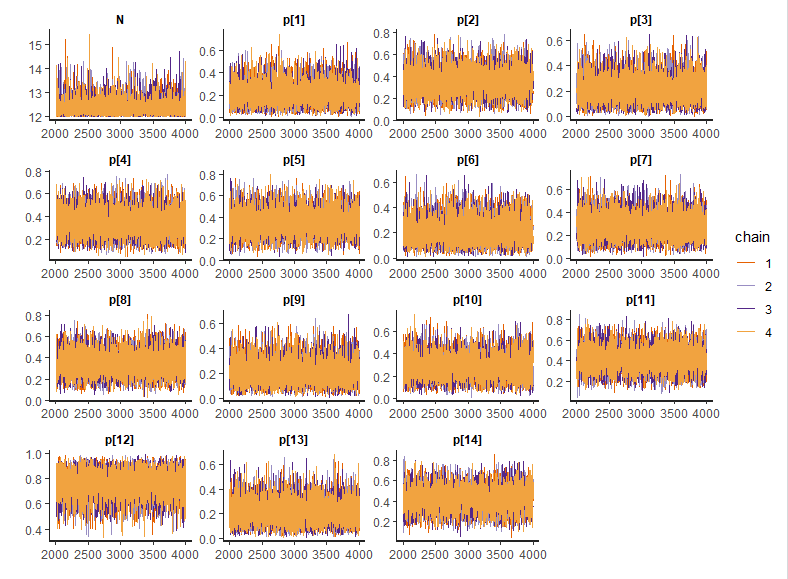
\includegraphics[width=16cm,height=10cm]{imgs/stan_print.png}}

  \captionsetup{font=footnotesize,width=15cm}
  \caption{\small Cadeias geradas pelo código implementado em STAN.}
\end{figure}
\newpage
\section{Comentários}
Foi muito interessante realizar esse trabalho, a etapa de gibbs foi relativamente tranquila de se realizar, grande parte do foco ficou em achar uma solução na implementação. troquei ideias com a Aurora e Yohana sobre possíveis soluções e acabei chegando na solução de usar a aproximação Poisson-Normal.
Após encontrar essa possível solução optei por implementar primeiramente no STAN pois achei que seria mais fácil e de fato foi, durante a implementação no R tive alguns problemas principalmente com o espaço paramétrico de $\mathbf{p}$.




\newpage
\bibliography{ref}
\section*{Apêndice A}
\subsection*{A.1 Implementação Gibbs Sampler}
\begin{lstlisting}[language=R]
library(readr)
library(tidyverse)
dados <- read_table("./Atividade1/resolucao/dados.txt", 
                    col_names = FALSE)
colnames(dados) <- c('onca',paste0('armadilha',1:14))
nj <- dados%>%
  pivot_longer(-onca,values_to = "capturada",
               names_to = "armadilha",names_prefix = 'armadilha',
               names_transform = list(armadilha = as.numeric))%>%
  group_by(armadilha)%>%
  summarise(nj=sum(capturada))
mj <- dados%>%
  pivot_longer(-onca,values_to = "capturada",names_to = "armadilha",
               names_prefix = 'armadilha',
               names_transform = list(armadilha = as.numeric))%>%
  group_by(onca)%>%
  mutate(mj=case_when(cumsum(capturada)*capturada>1 ~ 1 , TRUE ~ 0))%>%
  group_by(armadilha)%>%
  summarise(mj=sum(mj))
Ngibbs=10e4
iter0 <- c(rpois(1,50),runif(14))
chain <- matrix(0,ncol = Ngibbs,nrow=length(iter0))
chain[,1] <- iter0
rownames(chain) <- c("N",paste0("p",1:14))
lambda=50
r <- sum(nj$nj)-sum(mj$mj)
nj <- nj$nj 
for (i in 2:Ngibbs) {
  lambda_pos <- lambda * prod(1-chain[-1,i-1])
  N_i_plus_1 <- rpois(n=1,lambda = lambda_pos) + r
  chain[1,i] <- N_i_plus_1 
  for (j in 1:length(nj)) {
    aux <- rbeta(n = 1,shape1 = nj[j]+1,shape2 = N_i_plus_1-nj[j]+1)
    chain[j+1,i] <- aux
  }
}
\end{lstlisting}

\newpage
\subsection*{A.1 Implementação HMC no R}
\begin{lstlisting}[language=R]
library(mvtnorm)
U <- function(theta,r=12,ni){
  N <- theta[1]
  pi <- theta[2:length(theta)]
  Ux <- log(gamma(N+1))-log(gamma(N-r+1)) + sum(ni*log(pi)+(N-ni)*log(1-pi)) - .01*(N-50)^2
  return(-Ux)
}
K <- function(M,rho){
  .5*t(rho)%*%M%*%rho
}
dUdt <- function(theta,r=12,ni){
  N <- theta[1]
  pi <- theta[2:length(theta)]
  dUdp <- (N*pi-ni)/(pi*(1-pi))
  dUdN <- -(digamma(N+1)/gamma(N+1)) + (digamma(N-r+1)/gamma(N-r+1)) - sum(log(1-pi)) + .02*(N-50)
  grad <- c(dUdN,dUdp)
  return(grad)
}

iter=2000
sample <- matrix(0,nrow = iter,ncol=15)
colnames(sample) <- c("N",paste0("p",1:14))
sample[1,] <- c(15,runif(14))
M <- cor(gbs%>%select(N,p1:p14))
L=50;delta=.001
for (i in 2:iter) {
  rho0 <- theta0 <- matrix(0,nrow = L,ncol = 15)
  rho0[1,] <- rmvnorm(1, mean = rep(0,15), sigma = M)
  theta0[1,] <- sample[i-1,]
  #leapfrog
  for (j in 2:L) {
    rhotemp <- rho0[j-1,] - (delta/2)*dUdt(theta = theta0[j-1,],ni=nj)
    theta0[j,] <- theta0[j-1,] + delta*rhotemp
    rho0[j,] <- rhotemp - (delta/2)*dUdt(theta = theta0[j,],ni=nj)
  }
  alpha=min(1,exp( -U(theta = theta0[L,],ni=nj) + U(theta = theta0[1,],ni=nj)- K(M,rho0[L,]) + K(M,rho0[1,])))
  if(runif(1)<alpha){
    sample[i,] <- theta0[L,]
  }else{
    sample[i,] <- sample[i-1,]
  }
}
\end{lstlisting}
\newpage
\subsection*{A.1 Implementação STAN}
\begin{lstlisting}[language=c]
data{
  int j;
  vector[j] ni;
  vector[j]mi;
}
transformed data{
  real r;  
  r = sum(ni) - sum(mi);
}
parameters{
  vector<lower=0.00001,upper=.9999>[j] p;
  real<lower=r> N;
}

transformed parameters{
  real Nt;
  Nt= N-r;
}

model{
  target+= normal_lpdf(Nt|50,sqrt(50));
  target+=uniform_lpdf(p|0,1);
  target += log(tgamma(N+1)) - log(tgamma(N - r + 1)) + sum(ni .* log(p)  + (N-ni).*log(1-p));
}

\end{lstlisting}


\end{document}
























